\documentclass[a4paper,11pt,oneside]{book}

\usepackage{etoolbox}

\makeatletter
\patchcmd{\@chapter}% <cmd>
	{\chaptermark{#1}}% <search>
	{\chaptermark{#1}%
	\addtocontents{loa}{\protect\addvspace{10\p@}}}% replace
	{}{}% <success><failure>
\makeatother

\usepackage{polyglossia}
\usepackage{fontspec}
\usepackage{csquotes}
\usepackage{geometry}
\usepackage[intlimits]{amsmath}
\usepackage{amsfonts}
\usepackage{amsthm}
\usepackage{graphicx}
\usepackage{indentfirst}
\usepackage{url}
\usepackage[backend=biber,style=iso-authoryear,sortlocale=cs_CZ,autolang=other,bibencoding=UTF8]{biblatex}
\usepackage{setspace}
\usepackage{hyperref}
\usepackage[ocgcolorlinks]{ocgx2}
\usepackage{braket}
\usepackage{enumerate}
\usepackage[chapter]{algorithm}
\usepackage{algorithmicx}
\usepackage{algpseudocode}
\usepackage{booktabs}
\usepackage{multirow}
\usepackage{float}

\geometry{tmargin=4cm,bmargin=3cm,lmargin=3cm,rmargin=2cm,headheight=0.8cm,headsep=1cm,footskip=0.5cm,marginparwidth=1.6cm}
\setdefaultlanguage{czech}
\setotherlanguage{english}
\setmainfont{TeX Gyre Termes}
\setcounter{secnumdepth}{3}
\addbibresource{zotero.bib}
\hypersetup{
	colorlinks,
	pdfencoding=auto,
	unicode=true,
	bookmarksopen=true,
	bookmarksopenlevel=3,
	citecolor=green,
	filecolor=blue,
	linkcolor=red,
	urlcolor=blue
}

% BibLaTeX fixes
\def\UrlBreaks{\do\/\do-}
\renewbibmacro{labeltitle}{}

\theoremstyle{plain}
\newtheorem{theorem}{Věta}[chapter]
\theoremstyle{definition}
\newtheorem{define}[theorem]{Definice}
\newtheorem{example}[theorem]{Příklad}
\theoremstyle{remark}
\newtheorem{remark}[theorem]{Poznámka}

\newcommand{\BPname}[1]{\textbf{#1}}
\newcommand{\BPenname}[1]{\textit{\textenglish{#1}}}

\newcommand{\BPspace}{\ensuremath{\mathcal}}
\newcommand{\BPfield}{\ensuremath{\mathbb}}
\newcommand{\BPset}{\ensuremath{\mathbb}}
\newcommand{\BPmat}{\ensuremath{\mathbf}}

\makeatletter
\renewcommand{\ALG@name}{Algoritmus}
\makeatother
\MakeRobust{\Call}
\algnewcommand\algorithmicparallelfor{\textbf{parallel for}}
\algdef{S}[FOR]{ParallelFor}[1]{\algorithmicparallelfor\ #1\ \algorithmicdo}
\algnewcommand\algorithmicbreak{\State\textbf{break}}
\algnewcommand\Break{\algorithmicbreak{}}

\newcommand{\result}[3]{%
	\begin{graph}[h]%
		\centering%
		\includegraphics[width=\textwidth]{images/results/#1}%
		\caption{#3}\label{#2}%
	\end{graph}%
}

\renewcommand{\listalgorithmname}{Seznam algoritmů}

\floatstyle{plain}
\newfloat{graph}{tbph}{logr}[chapter]
\floatname{graph}{Graf}

\usepackage{todonotes}


\begin{document}
\def\documentdate{7. července 2017}

\pagestyle{empty}

%\begin{center}
	\begin{minipage}{3cm}
		
\includegraphics[width=3cm,height=3cm,keepaspectratio]{images/titlepage/cvut}
	\end{minipage}
	\begin{minipage}{0.6\linewidth}
		\begin{center}
			\textsc{\large České vysoké učení technické v Praze}\\
			{\large Fakulta jaderná a fyzikálně inženýrská}
		\end{center}
	\end{minipage}
	\begin{minipage}{3cm}
		
\includegraphics[width=3cm,height=3cm,keepaspectratio]{images/titlepage/fjfi}
	\end{minipage}

	\vspace{3.3cm}

	\setstretch{1.75}\textbf{\huge Hierarchické modely síťového provozu}
	\vspace{1.1cm}

	\textenglish{\textbf{\huge Hierarchical models of network traffic}}
	\vspace{1.7cm}

	{\large Bakalářská práce}
\end{center}

\vfill

\begin{list}{}{
	\settowidth{\labelwidth}{MMMMMMMMM}
	\setlength{\leftmargin}{\labelwidth}
	\renewcommand{\makelabel}[1]{#1\hfil}}
	\item [{Autor:}] \textbf{Marek Dědič}
	\item [{Vedoucí práce:}] \textbf{Ing. Tomáš Pevný, Ph.D.}
	\item [{Konzultant:}] \textbf{Mgr. Petr Somol, Ph.D.}
	\item [{Akademický rok:}] 2016/2017
\end{list}


\cleardoublepage

%\null\vfill
%\begin{center}
	%- Zadání práce -
%\end{center}
%\vfill

%\newpage

%\null\vfill
%\begin{center}
	%- Zadání práce (zadní strana) -
%\end{center}
%\vfill

\cleardoublepage

%\noindent \textit{\Large Poděkování:}

\noindent Chtěl bych zde poděkovat především svému školiteli, doktoru Tomáši Pevnému,
za pečlivost, ochotu, vstřícnost a odborné i lidské zázemí při vedení
mé diplomové práce. Dále děkuji svému konzultantovi ................
za ................ (???)

\vfill

\noindent \textit{\Large Čestné prohlášení:}

\noindent Prohlašuji, že jsem tuto práci vypracoval samostatně a uvedl
jsem všechnu použitou literaturu.

\bigskip

\noindent V Praze dne \documentdate\hfill Marek Dědič

\vspace{2cm}


\cleardoublepage

%\begin{onehalfspace}
	\noindent \textit{Název práce:}

	\noindent \textbf{Hierarchické modely síťového provozu}
\end{onehalfspace}

\bigskip

\noindent \textit{Autor:} Marek Dědič

\bigskip

\noindent \textit{Obor:} Matematická informatika

\bigskip

\noindent \textit{Druh práce:} Bakalářská práce

\bigskip

\noindent \textit{Vedoucí práce:} Ing. Tomáš Pevný, Ph.D., Cisco systems, Inc.

\bigskip

\noindent \textit{Konzultant:} Mgr. Petr Somol, Ph.D., Cisco systems, Inc.

\bigskip

\noindent \textit{Abstrakt:}
Současné přístupy k detekci nežádoucího software sledováním síťového provozu klientů využívají ručně navržených příznaků jako části modelu. Tento přístup má několik nevýhod. Tato práce navrhuje plně automatický klasifikátor rozpoznávající aktivity malware na úrovni síťových spojení. K~tomu byl využit přístup pomocí multi-instančního učení. Součástí této práce je teoretické zavedení multi-instančního učení pomocí dvou rozdílných formalismů a shrnutí základních myšlenek dosavadních prací v oboru multi-instančního učení. Dále je popsána hierarchická struktura adresy URL jako vstupního objektu klasifikátoru. Je navržen model reflektující tuto inherentní strukturu a vysvětleno, jak využívá multi-instanční učení, v čem se liší a jak byl implementován pomocí umělých neuronových sítí. Jsou zde popsány metody sloužící k vyhodnocení kvality klasifikátoru a k porovnání s předchozím dílem. Navržený klasifikátor je porovnán s nejlepším předchozím modelem a je srovnán vliv jednotlivých parametrů modelu na jeho kvalitu.

\bigskip

\noindent \textit{Klíčová slova:}
detekce malware, klasifikace síťového provozu, model adresy URL, multi-instanční učení, učení se reprezentace, strojové učení

\vfill

\begin{english}
	\begin{onehalfspace}
		\noindent \textit{Title:}

		\noindent \textbf{Hierarchical models of network traffic}
	\end{onehalfspace}

	\bigskip

	\noindent \textit{Author:} Marek Dědič

	\bigskip

	\noindent \textit{Abstract:}
	\textenglish{The current approach to the detection of unwanted software by monitoring client traffic uses handwritten features as part of the model. This approach has several disadvantages. This thesis proposes a fully automated classifier which recognises malware activity at network connection level. The multi-instance learning approach was used in order to achieve this. As a part of this thesis the multi-instance learning was theoretically defined using two different formalisms and current work in this field was summarised. Subsequently, there was described the hierarchical structure of an URL address which was used as an input for the classifier. A model reflecting this inherent hierarchical structure was proposed and an explanation of how multi-instance learning was utilised and modified was presented together with the description of the implementation of the model using neural networks. Methods of classifier quality assessment were outlined. The classifier presented here was compared with prior art and the influence of model parameters on its quality was assessed.}

	\bigskip

	\noindent \textit{Keywords:}
	\textenglish{machine learning, malware detection, multi-instance learning, network traffic classification, representation learning, URL address model}

\end{english}


\cleardoublepage

\pagestyle{plain}

\listoftodos

\tableofcontents

\chapter*{Úvod}
\addcontentsline{toc}{chapter}{Úvod}

Co je to za problém, proč ho řeším, jaký je přístup k řešení


\pagestyle{headings}

\chapter{Řešená úloha}\label{problem}

Řešená úloha je problémem binární klasifikace, tedy problém, kdy je cílem zařadit objekty do jedné ze dvou tříd, jež nazýváme pozitivní a negativní. Tedy cílem je navrhnout vhodnou klasifikační funkci, který pro daný vstupní objekt určí příslušnou třídu. Vstupními objekty jsou v tomto případě adresy URL (srov. \cite{berners-lee_uniform_1994}). Příklad takovéto adresy je na obrázku \ref{url}. \BPname{Negativní třídou} se rozumí veškerý síťový provoz, který je součástí běžného provozu uživatele-klienta a jím spuštěných programů. \BPname{Pozitivní třídou} se rozumí síťový provoz který pochází z aktivit malware a nežádoucího software.

\begin{figure}[h]
	\centering
	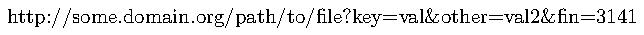
\includegraphics{images/url/url.pdf}
	\caption{Adresa URL}\label{url}
\end{figure}

Adresa URL se skládá z několika částí, mezi běžné patří \BPname{protokol} (\BPenname{protocol}), \BPname{doména} (\BPenname{domain} nebo \BPenname{host}), \BPname{port}, \BPname{cesta} (\BPenname{path}), \BPname{dotaz} (\BPenname{query} nebo \BPenname{searchpart}). Vzhledem k tomu, že protokolů je relativně málo a port se ve většině případů neudává, lze tyto dvě části pominout a zabývat se pouze doménou, cestou a dotazem.

\section{Struktura adresy URL}\label{URL_structure}

\cite{berners-lee_uniform_1994} definuje abecedu (dále označovanou \( \Sigma \)) všech možných znaků v adrese URL jako malá a velká písmena anglické abecedy, čísla a znaky \$ - \_ . + ! * ' ( ) , \% ; / ? : @ \& =. Každá adresa URL je pak slovem abecedy \( \Sigma \) (ne však naopak). Vybrané tři části adresy URL jsou definovány následovně.
\begin{define}
	\BPname{Doména} je podslovem adresy URL konstruovaným následovně: Pokud adresa URL obsahuje podslovo "://", doména začíná za tímto podslovem. V opačném případě doména začíná na záčátku adresy URL. Doména končí před prvním výskytem znaku "/" po začátku domény, případně na konci adresy URL, pokud tato už žádný znak "/" neobsahuje.
\end{define}
\begin{define}
	Pokud je doména sufixem adresy URL, je \BPname{cesta} definována jako prázdné slovo. V opačném případě je cesta definována jako podslovo adresy URL, začínající za znakem "/" ukončujícím doménu. Cesta končí před prvním výskytem znaku "?" po začátku cesty, případně na konci adresy URL, pokud tato už žádný znak "?" neobsahuje.
\end{define}
\begin{define}
	Pokud je doména nebo cesta sufixem adresy URL, je \BPname{dotaz} definován jako prázdné slovo. V opačném případě je dotaz definován jako sufix adresy URL, začínající za za znakem "?" ukončujícím cestu.
\end{define}

\begin{figure}[h]
	\centering
	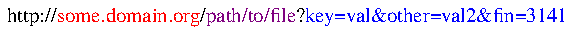
\includegraphics{images/url_parts/url_parts.pdf}
	\caption{Části adresy URL}\label{url_parts}
\end{figure}

Na obrázku \ref{url_parts} je příklad dělení adresy URL. Doména ja zvýrazněná červenou barvou, cesta fialovou a dotaz modrou.

Každá z těchto tří částí adresy URL se sama skládá z několika částí, zvaných \BPname{tokeny}. Doména se skládá z několika úrovní, lišících se obecností. Tyto tokeny jsou odděleny znakem ".". Cesta se skládá z názvů složek a souborů, které jsou dotazovány. Tyto tokeny jsou odděleny znakem "/". Dotaz je tvořen dvojicemi klíč--hodnota, oddělenými znakem "\&". Na obrázku \ref{url_subparts} je příklad tohoto rozdělení, v barvách korespondujících s obrázkem \ref{url_parts}, v různých odstínech pro různé tokeny.

\begin{figure}[h]
	\centering
	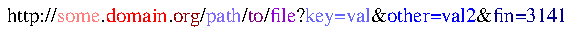
\includegraphics{images/url_subparts/url_subparts.pdf}
	\caption{Části a tokeny adresy URL}\label{url_subparts}
\end{figure}

Je zřejmé, že na pořadí tokenů domény záleží, definují "cestu" k cílovému serveru a jsou řazeny od nejkonkrétnější k nejobecnější (srov. \cite{mockapetris_domain_1987}). Stejně tak u cesty závisí na pořádí, které definuje adresářové umístění požadovaného souboru na serveru.

\section{Výhody přístupu pomocí MIL}

Klasifikační funkce byla odhadována pomocí tzv. \BPname{multi-instančního učení} (MIL)\footnote{resp. jeho speciální varianta, blíže popsaná v kapitole \ref{model}}, poprvé popsaného v \cite{dietterich_solving_1997}. Tento přístup, podrobněji popsaný v kapitole \ref{MIL}, vychází z předpokladu, že vzorek nelze reprezentovat vektorem o konstantní délce, ale sadou (dále zvanou \BPname{taška}) takovýchto vektorů (dále zvaných \BPname{instance}). Dále je pak předpokládáno, že každou tašku, obsahující neznámý počet instancí, je možno zařadit do nějaké třídy, přestože ne všechny její objekty náleží do této třídy. \todo{URL je taška} Adresu URL lze považovat za takovouto tašku za využití jejího hierarchického modelu, nastíněného v sekci \ref{URL_structure}. Proto lze přístup pomocí Multi-instančního učení aplikovat na tento problém.

Přístup pomocí Multi-instančního učení produkuje topologicky složitější modely než je srovnatelný model založený na ručně navržených příznacích. Výměnou za tuto nevýhodu v podobě zvětšené složitosti implementační je zmenšená složitost výpočetní. Multi-instanční model totiž modeluje každou instanci nejprve zvlášť a teprve poté následuje model pro celý vzorek. To v případě použití neuronové sítě znamená výrazně méné propojení než u srovnatelné plně propojené síťě se stejnými počty neuronů ve stejných vrstvách. Důležitým rozdílem též je, že narozdíl od tohoto modelu je multi-instanční model rozdělen do dvou částí (model pro instance a model pro tašky), přičemž ten samý instanční model je použit několikrát v rámci jedné tašky.

Multi-instanční přístup nám tedy dovoluje vytvořit model, jehož topologie odpovídá hierarchické struktuře adresy URL, je výpočetně méně náročný než srovnatelný klasický model a umožňuje znovupoužití některých částí. To jsou důvody, proč byl tento přístup zvolen.

\section{Trénovací a testovací data}\label{dataset}
\todo{Zkontrolovat}

K trénování a testování modelu byla použita data získaná z Cisco Cloud Web Security \todo{?}. Tato data představují záznamy HTTP provozu více jak 100 společností v šesti různých časových úsecích mezi listopadem 2013 a březnem 2015. Datový soubor je rozdělen na data určená k trénování a data určená k ověření kvality navržených klasifikátorů. Oba tyto soubory jsou dále rozděleny na dvě části, z nichž jedna obsahuje pouze legitimní provoz a druhá obsahuje směs legitimního provozu a provozu pocházejícího z činnosti malware. Toto rozdělení datového souboru je shrnuto v tabulce \ref{dataset_table}.

\begin{table}[h]
	\caption{Souhrn použitých souborů dat}\label{dataset_table}
	\centering
	\begin{tabular}{lrr}
		\toprule
		\null & \multicolumn{2}{c}{Počet adres} \\
		\cmidrule(l){2-3}
		Dataset & Legitimní & Malware \\
		\midrule
		Trénovací legitimní & 417 208 484 & 0 \\
		Trénovací směs & 17 390 889 & 34 359 733 \\
		Testovací legitimní & 1 522 255 052 & 0 \\
		Testovací směs & 2 855 992 & 4 051 944 \\
		\bottomrule
	\end{tabular}
\end{table}

\chapter{Multi-instanční učení}\label{MIL}

Co to je, definice z \cite{dietterich_solving_1997}.

Metody řešení - 3 paradigmata - IS, proč nevyhovuje, BS, ES. Co kdo kdy dělal.

Formalismus z \cite{pevny_using_2016}.

Proč embedded space? (výpočetně méně náročný než BS, neexistence instance-level labelů.)

Multi-instanční učení (anglicky \textenglish{\textit{multi-instance learning, MIL}}), poprvé takto popsané v \cite{dietterich_solving_1997}, je variací metody učení s učitelem (anglicky \textenglish{\textit{supervised learning}}), metody pro určení klasifikační funkce z trénovacích dat. Nechť existují vstupní objekty ze vstupního prostoru \( \BPspace X \), výstupní objekty z výstupního prostoru \( \BPspace Y \), kde každému \( x \in \BPspace X \) lze jednoznačně přiřadit \( y \in \BPspace Y \). Tyto výstupní objekty avšak nejsou známé ani pro trénovací data. Proto jsou vstupní objekty seskupeny do takzvaných tašek (anglicky \textenglish{\textit{bag}}).
\begin{define}
	Nechť \( \BPspace X \) je prostorem vstupních objektů. Potom prostorem tašek je množina \( \BPspace B \) splňující podmínky
	\begin{enumerate}
		\item \( \BPspace B \subset \mathcal P \left( \BPspace X \right) \)
		\item \( \left( \forall x \in \BPspace X \right) \left( \exists ! b \in \BPspace B \right) \left( x \in b \right) \)
	\end{enumerate}
	Prvky prostoru tašek se nazývají taškami.
\end{define}
\begin{define}\label{baglabel}
	Nechť \( \BPspace X \) je prostorem vstupních objektů, \( \BPspace Y \) je prostorem výstupních objektů, kde platí
	\[ \left( \forall x \in \BPspace X \right) \left( \exists ! y_x \in \BPspace Y \right) \]
	Nechť \( \BPspace B \) je prostorem tašek. Nechť je v prostoru \( \BPspace Y \) definována funkce maximum. Potom výstupním objektem příslušícím tašce \( b \in \BPspace B \) je
	\[ y_b = \max_{x \in b} \left( y_x \right) \in \BPspace Y \]
\end{define}

\section{Metody řešení multi-instančních úloh}

V následující sekci jsou popsány tři převládající přístupy k řešení Multi-instančních problémů, více k problematice srov. \cite{pevny_using_2016}.

\subsection{Paradigma prostoru instancí}
Je předpokládána existence výstupních objektů pro všechny vstupní objekty (odpovídající instancím), přestože tyto hodnoty nejsou známé. Pro každou tašku je pak předpokládána exitence výstupního objektu \( y_b \). Cílem metody je najít klasifikační funkci \( f : \BPspace X \to \BPspace Y \) a posléze určit
\begin{equation}
	y_b = \max_{x \in b} \left( f \left( x \right) \right)
\end{equation}

\subsection{Paradigma prostoru tašek}
Předpoklady úlohy jsou omezeny pouze na existenci výstupních objektů na úrovni tašek. Lze definovat kernel funkci
\begin{equation}
	k : \BPspace B \times \BPspace B \to \BPfield R_0^+
\end{equation}
kterou je možno použít jako metriku při klasifikaci například algoritmem k-nejbližsích sousedů.

\subsection{Paradigma vloženého prostoru}
Předpoklady úlohy jsou (stejně jako u paradigmatu prostoru tašek) omezeny pouze na existenci výstupních objektů na úrovni tašek. Nechť existuje vkládající funkce \( \phi : \BPspace B \to \bar{\BPspace X} \), kde \( \bar{\BPspace X} \) je nějaký vstupní prostor. Díky této funkci lze reprezentovat kažkou tašku vstupním objektem \( \phi \left( b \right) \in \bar{\BPspace X} \) a nasledně lze použít jakýkoliv algoritmus používaný při klasickém učení s učitelem. Pokud \( \BPspace X = \bar{\BPspace X} = \BPfield R^n \), pak je většinou kladena na \( \phi \) podmínka
\begin{equation}
	\left( \exists \psi : \BPfield R^k \to \BPfield R \right) \left( \phi \left( x^{(1)}, \dots, x^{(k)} \right) = \left( \psi \left( x_1^{(1)}, \dots, x_1^{(k)} \right), \dots, \psi \left( x_n^{(1)}, \dots, x_n^{(k)} \right) \right) \right)
\end{equation}

\section{Použitý formalismus}\label{used_formalism}
V následujících částech bude používáno \( \BPspace X = \BPfield R^n \), \( \BPspace Y = \left\{ -1, +1 \right\} \) a \( \BPspace B \subset \bigcup_{k = 1}^{\infty} \left( \BPfield R^n \right) ^k \). Prvky \( \BPspace X \) budou nazývány \textit{vektory příznaků}, prvky \( \BPspace Y \) budou nazývány \textit{značky}. Instance bude považována za \textit{pozitivní}, pokud je pozitivní její značka, a negativní jinak. Při použití definice \ref{baglabel} bude taška považována za pozitivní, pokud obsahuje alespoň jednu pozitivní instanci, a negativní, pokud obsahuje pouze negativní instance. Je použito paradigma vloženého prostoru a dále popsaný formalismus, převzatý z \cite{pevny_using_2016} a \cite{pevny_discriminative_2016}.

Nechť existuje prostor rozdělení pravděpodobnosti \( \BPspace P^{\BPspace X} \). Každá taška \( b \) je pak realizací nějaké pravděpodobnostní funkce \( P \left( p_b, y_b \right) \) kde \( p_b \in \BPspace P^{\BPspace X} \) je rozdělení pravděpodobnosti instancí v \( b \), a \( y_b \in \BPspace Y \) je značka této tašky. Je tedy předpokladem, že pravděpodobnostní funkce závisí i na značce, tj. \( p_+ \neq p_- \) kde \( p_+ \sim P(p, +1) \) a \( p_- \sim P(p, -1) \). Prostor všech tašek lze poté alternativně zapsat jako
\todo{Vyhovuje definici?}\begin{equation}
	\BPspace B = \left\{ \left\{ x_1, x_2, \dots, x_n \right\} \in \BPspace P \left( \BPspace X \right) \middle| \left( \forall i \in \hat n \right) \left( x_i \sim p \in \BPspace P^{\BPspace X} \right) \right\}
\end{equation}

Pokud jsou zvoleny funkce \( k : \BPspace X \to \BPspace X \) a \( g : \bigcup_{k = 1}^{\infty} \BPspace X^k \to \bar{\BPspace X} \), lze vkládající funkci definovat jako
\begin{equation}\label{net_pooling}
	\phi : \BPspace B \to \bar{\BPspace X} : b \mapsto g \left( \left\{ k \left( x \right) \middle| x \in b \right\} \right)
\end{equation}
Za \( g \) lze volit například funkce minimum, maximum, aritmetický průměr. Funkce \( k \) je potom určována algoritmem pro učení s učitelem. \todo{Obrázek z \cite{pevny_using_2016}}\todo{Zapsat lépe}Tedy neuronové síťě určující funkce \( f \) a \( k \) jsou trénovány najednou.

\chapter{Použitý model}\label{model}

Jelikož úloha představená v kapitole \ref{problem} je úlohou v níž je adresa URL rozdělena na části a ty jsou posléze rozděleny na tokeny, je na model použitý k aproximaci klasifikační funkce kladen požadavek, aby reflektoval tuto hierarchickou strukturu vstupních dat. Použitý model využívá přístupu pomocí multi-instančního učení \footnote{resp. jeho speciální varianty, popsané v kapitole \ref{MIL-modification}.}, popsaného v kapitole \ref{MIL}, aplikovaného dvakrát na sebe sama. Tím je umožněno modelovat nejprve tři vybrané části adresy URL (doménu, cestu a dotaz) z jejich tokenů, a posléze z těchto tří částí modelovat samotnou adresu URL. V následující kapitole je předpokládáná základní znalost fungování umělých neuronových sítí v rozsahu prvních dvou částí \cite{goodfellow_deep_2016}.

\section{Reprezentace adresy URL pomocí tašek vektorů}\label{URL_MIL_representation}
\todo{Přepsat bottom-up k čitelnosti.}V kapitole \ref{problem} byla definována abeceda všech znaků přípustných v adrese URL \( \Sigma \) jako abeceda malých a velkých písmen anglické abecedy, čísel a znaků \$ - \_ . + ! * ' ( ) , \% ; / ? : @ \& = (srov. \cite{berners-lee_uniform_1994}). Každá adresa URL, každá její část i každý token je slovem v abecedě \( \Sigma \). Aby však bylo možné s těmito objekty dále pracovat, je zapotřebí tato slova převést na vektory. Toho je dosáhnuto pomocí nějaké funkce \( \psi : \Sigma^* \to \BPfield R^n \) kde symbolem \( \Sigma^* \) je označována množina všech slov nad abecedou \( \Sigma \). Tím je definován prostor vstupních objektů, dále nazývaných \BPname{vektory příznaků} (\BPenname{feature vectors}), jako
\[ \BPspace X_1 = \psi \left( \Sigma^* \right) \subset \BPfield R^n \]
Tento prostor obsahuje všechny vektory příznaků odpovídající tokenům adresy URL. Prostor \( \BPspace B_1 \subset \BPspace P^M \left( \BPspace X_1 \right) \) je tedy konstruován tak, že každá taška v \( \BPspace B_1 \) odpovídá vektorům příznaků tokenů jedné části jedné adresy URL. Za použití paradigmatu vloženého prostoru, popsaného v kapitole \ref{embedded-space-paradigm} lze najít nějakou vkládající funkci
\[ \phi_1 : \BPspace B_1 \to \BPspace X_2 \]
kde \( \BPspace X_2 \) je opět nějaký vstupní prostor, který může, ale nemusí být totožný s \( \BPspace X_1 \). Nad tímto prostorem je konstruován prostor tašek \( \BPspace B_2 \subset \BPspace P^M \left( \BPspace X_2 \right) \) tak, že každá taška v prostoru \( \BPspace B_2 \) odpovídá vektorům příznaků tří částí jedné adresy URL. Znovupoužítím paradigmatu vloženého prostoru lze nalézt vkládající funkci
\[ \phi_2 : \BPspace B_2 \to \BPspace X_3 \]
kde \( \BPspace X_3 \) je opět nějaký vstupní prostor, který obecně nemusí být totožný s prostory \( \BPspace X_1 \) a \( \BPspace X_2 \). Tím je celá adresa URL vyjádřena jedním vektorem příznaků z prostoru \( \BPspace X_3 \). Celá tato abstrakce je graficky znázorněna na obrázku \ref{url_model_MIL}.

\begin{figure}[h]
	\centering
	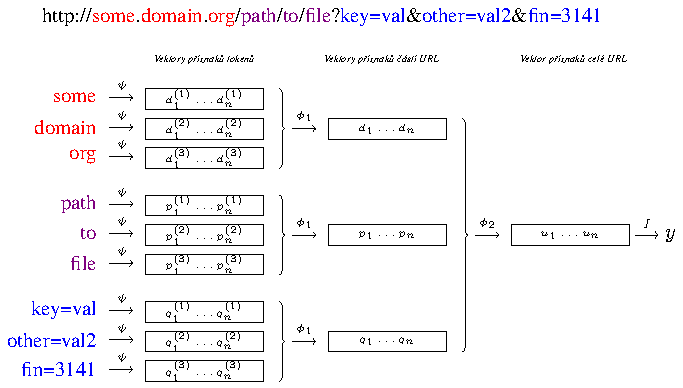
\includegraphics{images/model_MIL/model_MIL.pdf}
	\caption{Model adresy URL}\label{url_model_MIL}
\end{figure}

\section{Modifikace MIL pro tuto úlohu}\label{MIL-modification}
Každá adresa URL musí obsahovat doménu, avšak i adresy, kterým chybí cesta nebo dotaz (nebo dokonce cesta i dotaz), mohou být validními adresami URL ve smyslu \cite{berners-lee_uniform_1994}. Vzhledem k tomu, jak byl prostor \( \BPspace B_2 \) konstruován, je tedy zřejmé, že platí
\[ \left( \forall b \in \BPspace B_2 \right) \left( 1 \leq \left| b \right| \leq 3 \right) \]
Je ovšem možné chybějící části adresy URL reprezentovat jedním tokenem odpovídajícím prázdnému slovu abecedy \( \Sigma \) \footnote{Což nutně nemusí znamenat, že jsou reprezentovány nulovým vektorem příznaků.}. Díky tomuto rozšíření lze předchozí odhad velikosti tašek v prostoru \( \BPspace B_2 \) zesílit na
\[ \left( \forall b \in \BPspace B_2 \right) \left( \left| b \right| = 3 \right) \]

Protože doména, cesta a dotaz mají v adrese URL fundamentálně odlišný účel, nedává smysl, aby jim odpovídající vkládající funkce byly totožné. Rozšíření multi-instančního přístupu navržené v předchozím odstavci nám umožňuje nahradit funkci \( \phi_1 \) třemi různymi vkládajícími funkcemi \( \phi_D \), \( \phi_P \) a \( \phi_Q \), odpovídajícími doméně, cestě a dotazu respektive. Rovněž předpis pro vkládající funkci \( \phi_2 \) se díky konstantní velikosti tašek z prostoru \( \BPspace B_2 \) zjednoduší na
\[ \phi_2 : \BPspace X_2^3 \to \BPspace X_3 \]
Takto modifikovaná abstrakce je graficky znázorněna na obrázku \ref{url_model_modified_MIL}.

\begin{figure}[h]
	\centering
	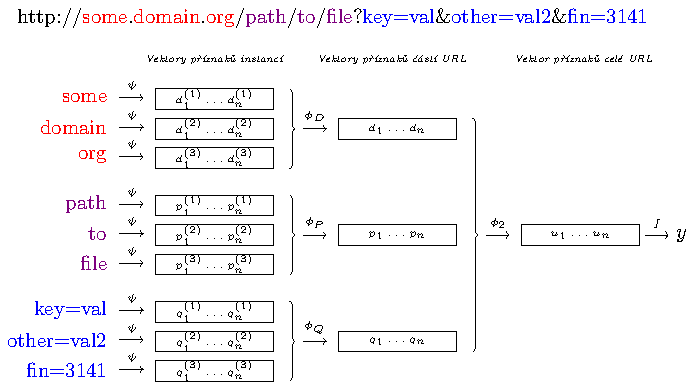
\includegraphics{images/model_modified_MIL/model_modified_MIL.pdf}
	\caption{Modifikovaný model adresy URL}\label{url_model_modified_MIL}
\end{figure}

\section{Metody hledání vkládající a klasifikační funkce}
Obecně lze v klasickém multi-instančním učení definovat vkládající funkci \( \phi \) jako
\begin{equation}\label{netpooling}
	\phi : \BPspace B \to \bar{\BPspace X} : b \mapsto g \left( \left\{ k \left( x \right) \middle| x \in b \right\} \right)
\end{equation}
kde \todo{obor hodnot k}
\begin{align*}
	k &: \BPspace X \to \BPspace X \\
	g &: \bigcup_{m = 1}^{+ \infty} \BPspace X^m \to \bar{\BPspace X}
\end{align*}
Za \( g \) lze volit napříkald funkce minimum, maximum, aritmetický průměr. Funkce \( k \) je definována neuronovou sítí, která je trénována libovolným algoritmem pro učení s učítelem. Pokud jsou funkce \( k \) a \( f \) obě definovány neuronovou sítí, jsou tyto neuronové sítě trénovány společně.

V dalším textu budou předpokládány již konkrétní prostory, a to sice
\begin{align*}
	\BPspace X_1 &= \BPfield R^n \\
	\BPspace X_2 &= \BPfield R^n \\
	\BPspace X_3 &= \BPfield R^{3n} \\
	\BPspace Y &= \left\{ -1, +1 \right\}
\end{align*}
pro nějaké \( n \in \BPfield N \).

Přístup pomocí \eqref{netpooling} byl využit pro vkládající funkce první úrovně, tedy
\begin{align*}
	\phi_D &: \BPspace B_1 \to \BPfield R^n : b \mapsto g_D \left( \left\{ k_D \left( x \right) \middle| x \in b \right\} \right) \\
	\phi_P &: \BPspace B_1 \to \BPfield R^n : b \mapsto g_P \left( \left\{ k_P \left( x \right) \middle| x \in b \right\} \right) \\
	\phi_Q &: \BPspace B_1 \to \BPfield R^n : b \mapsto g_Q \left( \left\{ k_Q \left( x \right) \middle| x \in b \right\} \right)
\end{align*}
Za vkládající funkci druhé úrovně byla volena funkce konkatenace vektorů, tedy funkce \( \phi_2 : \left( \BPfield R^n \right)^3  \to \BPfield R^{3n} \) s funkčním předpisem
\begin{multline}
	\phi_2 \left( \left( x_1^{(1)}, \dots, x_n^{(1)} \right), \left( x_1^{(2)}, \dots, x_n^{(2)} \right), \left( x_1^{(3)}, \dots, x_n^{(3)} \right) \right) = \\
	= \left( x_1^{(1)}, \dots, x_n^{(1)}, x_1^{(2)}, \dots, x_n^{(2)}, x_1^{(3)}, \dots, x_n^{(3)} \right)
\end{multline}
Takto lze vkládající funkci \( \phi_2 \) volit pouze díky modifikaci navržené v kapitole \ref{MIL-modification}.

Klasifikační funkce \( f : \BPfield R^{3n} \to \left\{ -1, +1 \right\} \) je definovaná neuronovou síťí, která je trénovaná společně s neuronovými sítěmi definujícími funkce \( k_D \), \( k_P \) a \( k_Q \).

Takto navržené vkládající funkce zanedbávají pořadí objektů v jednotlivých taškách. Tento přístup byl pro svou jednoduchost zvolen, přestože pořadí objektů v taškách má vliv na výsledný klasifikátor (srov. \cite{vinyals_order_2015}).

\section{Použité přenosové funkce}
\todo{Zavést písmenka v textu - x, W, b}V modelech požitých k řešení úlohy popsané v kapitole \ref{problem} byly použity tři typy neuronů s různými \BPname{přenosovými funkcemi} (\BPenname{activation function}).

\subsection{Lineární přenosová funkce}
Jedním z nejjednoduších typů neuronů je neuron s lineární přenosovou funkcí, mající tvar (bez váhy a vychýlení)
\[ f : \BPfield R \to \BPfield R : x \mapsto x \]

\subsection{ReLU}
Neurony typu \BPname{ReLU} (\BPenname{Rectified linear unit}) používají přenosovou funkci (bez váhy a vychýlení)
\[ f : \BPfield R \to \BPfield R : x \mapsto \max \left\{ 0, x \right\} \]

\subsection{Maxout}
Pro neurony typu \BPname{maxout} (srov. \cite{goodfellow_maxout_2013}) nelze přenosovou funkci definovat stejně jednoduše jako v případě neuronů typu ReLU. Přenosová funkce \( h \) v tomto případě nebývá definována pro jednotlivé neurony, ale pro celou vrstvu neuronů po složkách \( h_i : \BPfield R^n \to \BPfield R \) jako funkce (včetně váhy a vychýlení)
\[ h_i \left( x \right) = \max_{j \in \left[ 1, k \right]} z_{ij} \]
kde
\[ z_{ij} = x^T \BPmat W_{\cdot ij} + b_{ij} \]
kde
\[ \BPmat W \in \BPfield R^{n, m, k} \qquad b \in \BPfield R^{m, k} \]
Lze tedy vrstvu maxout chápat jako \( k \) lineárních vrstev, z nichž je vybráno maximum výstupu.

\subsection{Softmax}
Přenosová funkce pro neurony typu \BPname{softmax} je taktéž definována pro celou prstvu po složkách \( h_i : \BPfield R^n \to \BPfield R \) jako funkce (bez váhy a vychýlení)
\[ h_i \left( x \right) = \frac{e^{x_i}}{\sum_{j = 1}^n e^{x_j}} \]

\todo{Loss funkce}

\section{Metody trénování neuronových sítí}
Jednou ze základních metod trénování neuronových sítí je metoda \BPname{gradientního sestupu} (srov. \cite{cauchy_methode_1847}). Předpokládá se existence nějaké objektivní funkce \( J \left( \theta \right) \), jejíž minimum je hledáno. \( \theta \in \BPfield R^d \) jsou učené parametry modelu. Tyto parametry se opakovaně mění, dokud není nalezeno požadované minimum funkce \( J \). Metoda gradientního sestupu počítá nové parametry \( \hat \theta \) jako
\[ \hat \theta = \theta - \eta \nabla_{\theta} J \left( \theta \right) \]
kde \( \eta \) je krok učení. Metoda \BPname{stochastického gradientního sestupu} provádí tuto korekci pro každou dvojici vstupního objektu \( x \) a výstupního objektu \( y \), tedy jde o metodu tvaru
\[ \hat \theta = \theta - \eta \nabla_{\theta} J \left( \theta; x, y \right) \]
Výhodou této metody je efektivita učení při velkém množství trénovacích dat, avšak její nevýhodou je velká fluktuace hodnot objektivní funkce.

\todo{Mini-batch SGD}

Metoda stochastického gradientního sestupu je základem pro mnoho moderních metod trénování neuronových sítí (srov. \cite{duchi_adaptive_2011}, \cite{zeiler_adadelta:_2012}, \cite{tieleman_lecture_2012} a \cite{kingma_adam:_2014}). Použitá metoda je další metodou založenou na gradientním sestupu, ADAM.

\BPname{ADAM} (srov. \cite{kingma_adam:_2014}) je variantou stochastického gradientního sestupu s proměnlivým krokem učení. K správnému nastavení tohoto kroku je v této metodě přenášena hodnota gradientu a jeho čtverce mezi jednotlivými kroky. Metoda ADAM je parametrizována třemi parametry \( \beta_1 \), \( \beta_2 \) a \( \varepsilon \). V každém kroku \( t \) jsou počítány momenty
\[ m_t = \beta_1 m_{t - 1} + \left( 1 - \beta_1 \right) \nabla_{\theta} J \left( \theta \right) \]
\[ v_t = \beta_2 v_{t - 1} + \left( 1 - \beta_2 \right) \left( \nabla_{\theta} J \left( \theta \right) \right)^2 \]
Vzhledem k tomu, že počáteční hodnoty jsou \( m_0 = 0 \) a \( v_0 = 0 \), bylo by učení zpočátku velice pomalé. Tomu je předejito použitím opravných hodnot
\[ \hat{m_t} = \frac{m_t}{1 - \beta_1^t} \]
\[ \hat{v_t} = \frac{v_t}{1 - \beta_2^t} \]
Nová hodnota parametrů modelu je pak nalezena jako
\[ \hat \theta = \theta - \frac{\eta \hat{m_t}}{\sqrt{\hat{v_t}} + \varepsilon} \]
\cite{kingma_adam:_2014} navrhují hodnoty parametrů metody
\[ \beta_1 = 0.9 \qquad \beta_2 = 0.999 \qquad \varepsilon = 10^{-8} \]

Metoda ADAM byla vybrána z důvodů použití adaptivního kroku učení, vedoucího ke stabilnější výsledné hodnotě a počáteční rychlosti díky využití opravných hodnot. Mezi další výhody patří jednoduché použití díky dobře fungujícím hodnotám parametrů, které byly navrženy autory metody.

\chapter{Metody vyhodnocení}

Úloha popsaná v kapitole \ref{problem} je úlohou \BPname{binární klasifikace}. To znamená, že jejím cílem je zařadit vstupní objekty do jedné ze dvou tříd, označovaných jako pozitivní a negativní. Předpokládá se existence nějaké klasifikační funkce \( f : \BPspace X \to \left\{ -1, +1 \right\} \), která pro každý vstupní objekt určí příslušnou třídu, symbolizovanou hodnotou \( -1 \) nebo \( +1 \). Model popsaný v kapitole \ref{model} se snaží tuto neznámou klasifikační funkci aproximovat. Za účelem zhodnocení kvality této aproximace je v této kapitole nejprve zavedeno několik pojmů vztahujících se k binární klasifikaci a následně popsáno několik metod vizualizace kvality binárních klasifikátorů. \todo{Zkontrolovat po napsání}

\begin{define}
	Nechť \( r \in \left\{ -1, +1 \right\} \) je správným výsledkem pro nějaký vstupní objekt v úloze binární klasifikace. Nechť \( p \in \left\{ -1, +1 \right\} \) je aproximací \( r \). Odhad \( p \) nazýváme
	\begin{enumerate}[i.]
		\item \BPname{Pozitivní} (\BPenname{Prediction positive}) pokud \( p = +1 \).
		\item \BPname{Negativní} (\BPenname{Prediction negative}) pokud \( p = -1 \).
		\item \BPname{Pravdivě pozitivní} (\BPenname{True positive}) pokud \( r = +1 \land p = +1 \).
		\item \BPname{Pravdivě negativní} (\BPenname{True negative}) pokud \( r = -1 \land p = -1 \).
		\item \BPname{Falešně pozitivní} (\BPenname{False positive}) pokud \( r = -1 \land p = +1 \).
		\item \BPname{Falešně negativní} (\BPenname{False negative}) pokud \( r = +1 \land p = -1 \).
	\end{enumerate}
	Falešně pozitivní odhad je také nazýván \BPname{chybou prvního druhu}, falešně negativní odhad je také nazýván \BPname{chybou druhého druhu}.
\end{define}

\todo{Nechcete sem dat takovou tu obvyklou tabulku }

\section{Indikátory kvality binárního klasifikátoru}\label{quality_indicators}
Cílem jakéhokoliv odhadu v úloze binární klasifikace je minimalizovat počet falešně pozitivních a falešně negativních odhadů. Ne vždy je ale možné minimalizovat obě tyto hodnoty a je třeba o nich uvažovat vždy najednou -- aproximace, která označí všechny objekty jako pozitivní nebude mít žádné falešně negativní odhady, ale v praxi nemá takováto aproximace žádnou hodnotu \todo{Jak jinak říct, že je na nic?}. Obdobně aproximace označující všechny objekty za negativní nebude produkovat žádné falešně pozitivní odhady, ale opět to není vhodná aproximace. -- Aby tedy bylo možno uvažovat o kvalitě nějakého binárního klasifikátoru, jsou dále zavedeny některé \BPname{indikátory kvality} \todo{To jsem si vymyslel, není pro to nějaký termín?}.

\todo{Ja bych se tady rozepsal, cim jsou ty jednotlive miry inspirovane a proc byli zavedene.}

\begin{define}
	Nechť \( tp \) je počet pravdivě pozitivních odhadů nějakého binárního klasifikátoru na daném souboru dat. Nechť \( pp \) je celkový počet pozitivních odhadů tohoto binárního klasifikátoru (tedy počet pravdivě pozitivních a falešně pozitivních). Jako \BPname{přesnost} (\BPenname{precision}) tohoto klasifikátoru je označována hodnota
	\[ precision = \frac{tp}{pp} \]
\end{define}

\begin{define}
	Nechť \( tp \) je počet pravdivě pozitivních odhadů nějakého binárního klasifikátoru na daném souboru dat. Nechť \( rp \) je celkový počet pozitivních vzorků v datovém souboru (tedy počet pravdivě pozitivních a falešně negativních). Jako \BPname{odezva} (\BPenname{recall}) tohoto klasifikátoru je označována hodnota
	\[ recall = tpr = \frac{tp}{rp} \]
	Odezva je také nazývána \BPname{pravdivě pozitivní mírou} (\BPenname{true positive rate}).
\end{define}

\begin{define}
	Nechť \( fp \) je počet falešně pozitivních odhadů nějakého binárního klasifikátoru na daném souboru dat. Nechť \( rn \) je celkový počet negativních vzorků v datovém souboru (tedy počet pravdivě negativních a falešně pozitivních). Jako \BPname{falešně pozitivní míra} (\BPenname{false positive rate}) tohoto klasifikátoru je označována hodnota
	\[ fpr = \frac{fp}{rn} \]
\end{define}

\begin{define}
	Nechť \( fn \) je počet falešně negativních odhadů nějakého binárního klasifikátoru na daném souboru dat. Nechť \( rp \) je celkový počet pozitivních vzorků v datovém souboru (tedy počet pravdivě pozitivních a falešně negativních). Jako \BPname{falešně negativní míra} (\BPenname{false negative rate}) tohoto klasifikátoru je označována hodnota
	\[ fnr = \frac{fn}{rp} \]
\end{define}

\begin{define}
	Nechť \( precision \) je přesnost nějakékého binárního klasifikátoru a \( recall \) je jeho odezva. Jako \BPname{F-skóre} či také \BPname{F\textsubscript{1} skóre} tohoto klasifikátoru je označován harmonický průměr jeho přesnosti a odezvy, tedy
	\[ F_1 = 2 \, \frac{precision \cdot recall}{precision + recall} \]
\end{define}

\begin{theorem}\label{tpr+fnr}
	Platí
	\[ tpr + fnr = 1 \]
\end{theorem}

\todo{Název?}\section{Spojitá aproximace binárního klasifikátoru}\label{continuous_aprox}

Přestože v úloze binární klasifikace jsou objekty zařazované do jedné ze dvou tříd, může nastat případ, kdy aproximace klasifikační funkce má jiný obor hodnot než množinu \( \left\{ -1, +1 \right\} \). V obecném případě může být oborem hodnot této aproximace celý obor \( \BPfield R \). Je tedy třeba rozhodnout, které hodnoty binárního klasifikátoru budou považovány za pozitivní a které za negativní. Zřejmě se nabízí přístup, kdy je stanoven nějaký práh a všechny hodnoty vyšší než tento práh jsou považovány za pozitivní odhad, všechny hodnoty nižší než tento práh jsou považovány za negativní odhad. Indikátory kvality lze poté chápat jako funkce takovéhoto prahu. Volba správného prahu ovšem není triviálním úkolem.

Jedním z možných řešení problému volby prahu je přístup pomocí určování hodnoty indikátorů kvality binárního klasifikátoru pro všechny možné prahy. Vzhledem k předpokladu konečnosti klasifikovaného souboru dat jsou tyto indikátory (považované za funkce prahu) po částech konstantní a tedy postačuje je vyhodnotit v konečně mnoha bodech. Pro velké datasety (například dataset popsaný v kapitole \ref{dataset}) avšak ani toto není výpočetně možné. Zvoleným řešením je nalézt kvantily všech možných hodnot prahu a vyhodnotit indikátory kvality v těchto bodech.

\section{Křivky zobrazující vlastnosti binárního klasifikátoru}\label{evaluation_curves}
V následující podkapitole jsou popsány 4 křivky, pomocí kterých lze vizualizovat vlastnosti binárních klasifikátorů. V celé podkapitole jsou indikátory kvality považovány za funkce prahu.

\subsection{PR křivka}
\BPname{PR křivka} (\BPenname{Precision-Recall curve}) je křivkou zobrazující vztah mezi přesností a odezvou klasifikátoru pro různé prahy. PR křivka grafem množiny
\[ \left\{ \left( recall \left( x \right), precision \left( x \right) \right) \middle| x \in \BPfield R \right\} \]
Jde tedy o obor hodnot funkce \( \BPfield R \to \BPfield R^2 \), nikoliv o graf funkce \( \BPfield R \to \BPfield R \).

\subsection{ROC křivka}
\BPname{ROC křivka} (\BPenname{Receiver operating characteristic curve}) je křivkou zobrazující vztah mezi falešně pozitivní mírou a pravdivě pozitivní mírou klasifikátoru pro různé prahy. ROC křivka grafem množiny
\[ \left\{ \left( fpr \left( x \right), tpr \left( x \right) \right) \middle| x \in \BPfield R \right\} \]
V grafu ROC křivky je vyznačena i množina všech bodů \( \left( x, x \right) \), neboť náhodně volená klasifikační funkce by měla ROC křivku blízkou takovéto množině. Osa X grafu ROC křivky je v logaritmickém měřítku.

\subsection{DET křivka}
\BPname{DET křivka} (\BPenname{Detection error tradeoff curve}, srov. \cite{martin_det_1997}) je modifikací ROC křivky. DET křivka je grafem množiny
\[ \left\{ \left( fpr \left( x \right), fnr \left( x \right) \right) \middle| x \in \BPfield R \right\} \]
Z věty \ref{tpr+fnr} je zřejmé, že DET křivka je ROC křivkou otočenou podle osy Y \todo{Zdůraznit, že v bodě 0.5?}. Rozdílem ovšem je měřítko, v jakém je tato křivka vykreslována. Na obě osy grafu je aplikována funkce
\[ q \left( x \right) = \sqrt{2} \cdot erf^{-1} \left( 2x - 1 \right) \]
kde
\[ erf \left( x \right) = \frac{1}{\sqrt{\pi}} \int_{-x}^{x} e^{-t^2} \mathrm{d} t \]

\subsection{Křivka F-skóre}
Křivka F-skóre je grafem funkce \( x \mapsto F_1 \left( x \right) \).

\section{Proč vlastní implementace?}
K výpočtu křivek popsaných v kapitole \ref{evaluation_curves} bylo vyzkoušeno několik softwarových balíčků dostupných pro jazyk Julia (\cite{zea_roc.jl:_2015}, \cite{leeuwen_rocanalysis.jl:_2016} a \cite{lin_mlbase.jl:_2017}). Všechny tyto balíčky avšak neumožňovaly výpočet indikátorů kvality z důvodů příliš vysoké výpočetní náročnosti či paměťové náročnosti. Všechny tyto balíčky rovněž neumožňují paralelní výpočet indikátorů kvality. Proto byl navržen vlastní balíček s názvem EduNetsEvaluate.jl, který umožňuje výpočet indikátorů kvality popsaných v kapitole \ref{quality_indicators} i pro soubory dat tak velké jako ten, popsaný v kapitole \ref{dataset}. Výpočet všech indikátorů kvality je z velké části paralelizovaný, což umožňuje plně využít výpočetní kapacity moderních vícejádrových procesorů a procesorů využívajících technologii Hyper-threading.

\section{Implementace}
Následující podkapitola obsahuje přehled metod použitých k implementaci paralelního výpočtu PR křivky a ROC křivky.

Vzhledem k tomu, že použitý dataset je rozdělen do mnoha souborů, je možné každý takovýto soubor zpracovat zvlášť a následně agregovat výsledky. O velké části souborů je známo, že obsahují pouze objekty negativní třídy. Pokud je předpokládáno, že všechny objekty jsou seřazené podle hodnoty jejich předpovědi, při postupném procházení se při přechodu od negativního objektu k následujícímu negativnímu objektu nezmění hodnota odezvy. Tedy pokud bude PR křivka počítána pouze z pozitivních objektů, na její tvar to nebude mít žádný vliv. Pro ROC křivku platí stejné pozorování. Tím je umožněn výpočet vhodných hodnot prahů (ve smyslu kapitoly \ref{continuous_aprox}) pouze ze souborů, v nichž jsou nějaké pozitivní objekty. Tento výpočet je popsán v algoritmu \ref{thresholds}.

\begin{algorithm}
	\caption{Výpočet prahů}
	\label{thresholds}
	\begin{algorithmic}
		\Require $ mixed\_files $ \Comment Soubory obsahující pozitivní i negativní objekty
		\Statex
		\State $ thresholds \gets \Call{array}{} \left[ \, \right] \left[ \Call{size}{mixed\_files} \right] $ \Comment Pole polí
		\ParallelFor{$ file \in mixed\_files $}
			\State $ thresholds \left[ \, \right] \gets \Call{get\_predicted}{file} $
		\EndFor
		\State $ thresholds \gets \Call{concatenate}{thresholds} $
		\State $ thresholds \gets \Call{quantiles}{thresholds} $
	\end{algorithmic}
\end{algorithm}

Následně lze spočítat odezvu binárního klasifikátoru, k jejímuž výpočtu opět postačují pouze soubory, obsahující nějaké pozitivní objekty. Paralelizace tohoto výpočtu je umožněná	přístupem, kdy pro každý soubor je spočítán celkový počet pozitivních objektů v souboru a pro každý práh počet pravdivě pozitivních odhadů. Tyto hodnoty jsou poté sečteny přes všechny soubory a na jejich základě je spočítána odezva. Tento výpočet je popsán v algoritmu \ref{recall}. Pro výpočet přesnosti je již potřeba zohlednit všechny soubory včetně těch, které obsahují pouze negativní objekty. Pro každý soubor je zvlášť spočítán počet pravdivě pozitivních odhadů a celkový počet pozitivních odhadů. Tyto hodnoty jsou poté sečteny přes všechny soubory a na jejich základě je spočítána přesnost. Tento výpočet je analogický s výpočtem odezvy. 

\begin{algorithm}
	\caption{Výpočet odezvy}
	\label{recall}
	\begin{algorithmic}
		\Require $ mixed\_files $ \Comment Soubory obsahující pozitivní i negativní objekty
		\Require $ thresholds $
		\Statex
		\State $ RP \gets \Call{array}{} \left[ \Call{size}{mixed\_files} \right] $ \Comment Pole čísel
		\State $ TP \gets \Call{array}{} \left[ \Call{size}{thresholds} \right] \left[ \Call{size}{mixed\_files} \right] $ \Comment Pole polí
		\ParallelFor{$ file \in mixed\_files $}
			\State $ RP \left[ \, \right] \gets \Call{get\_real\_positives}{file} $
			\State $ TP \left[ \, \right] \gets \Call{get\_true\_positives}{file, thresholds} $
		\EndFor
		\State $ RP \gets \sum RP $
		\State $ TP \gets element-wise \sum TP $
		\State $ recall = \frac{TP}{RP} $
	\end{algorithmic}
\end{algorithm}

Pokud jsou objekty nejprve seřazeny podle hodnoty jejich předpovědi, lze poté počet pravdivě pozitivních i počet pozitivních odhadů počítat s asymptotickou složitostí \( \mathcal O \left( n \right) \), což spolu se složitostí řazení dává celkovou asymptotickou složitost \( \mathcal O \left( n \log n \right) \). Tento způsob efektivního výpočtu počtu pravdivě pozitivních odhadů je popsán v algoritmu \ref{TP}.

\begin{algorithm}
	\caption{Výpočet počtu pravdivě pozitivních odhadů se složitostí \( \mathcal O \left( n \right) \)}
	\label{TP}
	\begin{algorithmic}
		\Require $ predicted $ \Comment Odhady pro nějaký soubor objektů, seřazené vzestupně
		\Require $ real $ \Comment Skutečné třídy pro tento soubor ve stejném pořadí
		\Require $ thresholds $
		\Statex
		\State $ TP \gets \Call{array}{} \left[ \Call{size}{thresholds} \right] $
		\State $ TPcounter \gets \Call{count\_positives}{real} $
		\State $ THcounter \gets 1 $
		\For{$ i \gets 1 \; \text{to} \; \Call{size}{thresholds} $} \Comment Odhady menší než nejmenší z prahů
			\If{$ predicted \left[ 1 \right] < thresholds \left[ THcounter \right] $}
				\Break
			\EndIf
			\State $ TP \left[ THcounter \right] \gets TPcounter $
				\State $ THcounter \gets THcounter + 1 $
		\EndFor
		\If{$ real \left[ 1 \right] = +1 $}
			\State $ TPcounter \gets TPcounter - 1 $
		\EndIf
		\State $ j \gets 1 $
		\While{$ j < \Call{size}{predicted} - 1 $} \Comment Odhady mezi nejmenším a největším prahem
			\If{$ predicted \left[ j \right] < thresholds \left[ THcounter \right] \land predicted \left[ j + 1 \right] \geq thresholds \left[ THcounter \right] $}
				\State $ TP \left[ THcounter \right] \gets TPcounter $
				\State $ THcounter \gets THcounter + 1 $
			\Else
				\If{$ real \left[ j + 1 \right] = +1 $}
					\State $ TPcounter \gets TPcounter - 1 $
				\EndIf
				\State $ j \gets j + 1 $
			\EndIf
		\EndWhile
		\For{$ i \gets THcounter \; \text{to} \; \Call{size}{TP} $} \Comment Odhady větší než největší z prahů
			\State $ TP \left[ i \right] = 0 $
		\EndFor
	\end{algorithmic}
\end{algorithm}

Výpočet celkového počtu pozitivních odhadů je obdobný. Ve skutečné implementaci jsou tyto hodnoty počítány kvůli vyšší efektivitě najednou. Ze stejného důvodu je najednou počítána i přesnost s odezvou. Výpočet ROC křivky je obdobný jako výpočet PR křivky.

K výpočtu křivky F-skóre jsou využity hodnoty vypočítané pro PR křivku. K výpočtu DET křivky jsou využity hodnoty vypočítané pro ROC křivku a věta \ref{tpr+fnr}.

\chapter{Výsledky}

\section{Srovnání s nejlepším předchozím modelem}\label{prior_art_comparison}
Obrázek \ref{prior_art} srovnává PR křivky nejlepšího modelu (srovnání parametrů v následujících podkapitolách) s nejlepším předchozím modelem pro soubor dat popsaný v kapitole \ref{dataset} (srov. \cite{machlica_learning_2017}). Nejlepší model má vstupní vektor příznaků o délce 2053, příznaky jsou generované z trigramů. Všechny tři funkce operující na úrovní částí adresy URL jsou shodně realizovány jednou vrstvou 20 neuronů s přenosovou funkcí ReLU, následovanou agregací tašky funkcí aritmetického průměru. Funkce operující na úrovni celé adresy URL obsahuje jednu vrstvu 60 neuronů s lineární přenosovou funkcí, následovanou výstupní vrstvou 2 neuronů s přenosovou funkcí softmax. Síť byla učena metodou ADAM minimalizující cross-entropii, ukončenou po 25 000 krocích. Váha na pozitivní třídě byla 0.5. Mini-batch obsahovaly 100 pozitivních a 100 negativních vzorků. Srovnávaný předchozí model využívá rozšířenou nepublikovanou sadu 557 příznaků z \cite{machlica_learning_2017}. Model obsahoval 3 vrstvy 128 neuronů typu ReLU, následované výstupní vrstvou 2 neuronů s přenosovou funkcí softmax. Síť byla učena metodou ADAM minimalizující cross-entropii, ukončenou po 100 000 krocích. Váha na pozitivní třídě byla 0.5. Mini-batch obsahovaly 1000 pozitivních a 1000 negativních vzorků. Všechny křivky v této kapitole byly počítány s~kvantilizací pomocí percentilů (ve smyslu kapitoly \ref{continuous_aprox}).

\result{prior_art_PR.pdf}{prior_art}{Srovnání PR křivek s nejlepším předchozím modelem}

\section{Srovnání vlivu topologie sítě}

Bylo vyzkoušeno 5 různých topologií neuronových sítí, odpovídajících modelu popsanému v kapitole \ref{model}. Všechny tyto topologie používají tři identické neuronové sítě realizující funkce na úrovni částí adresy URL. Topologie označované jako \BPname{relumean}, \BPname{relurelumean}, \BPname{maxout3mean} a \BPname{maxout3maxout3mean} shodně realizují klasifikační funkci na úrovni celé adresy URL jednou vrstvou neuronů s lineární přenosovou funkcí a jednou vrstvou s přenosovou funkcí softmax. Topologie relumean používá pro funkce na úrovni částí adresy URL jednu vrstvu typu ReLU, následovanou agregační funkcí aritmetického průměru. Topologie relurelumean používá dvě vrstvy typu ReLU následované agregační funkcí aritmetického průměru. Topologie maxout3mean používá jednu vrstvu typu maxout3 (tj. maxout s parametrem \( k = 3 \)) následovanou agregační funkcí aritmetického průměru. Topologie maxout3maxout3mean využívá 2 vrstvy typu maxout3 následované agregační funkcí aritmetického průměru. Topologie \BPname{relurelumeanrelu} má funkce na úrovni částí adresy URL shodné s topologií relurelumean, avšak funkci na úrovni celé adresy URL realizuje jako jednu vrstvu typu ReLU následovanou jednou vrstvou s lineární přenosovou funkcí následovanou jednou vrstvou typu softmax. Ostatní parametry jsou shodné s parametry popsanými v kapitole \ref{prior_art_comparison}. PR křivky všech těchto topologií jsou zobrazeny na obrázku \ref{topologies}. \todo{Grafy v TikZ, aby byly stejné fonty, možná 2 vedle sebe. legenda na dobrém místě, české legendy}

\result{topology_PR.pdf}{topologies}{Srovnání PR křivek různých topologií}

\section{Srovnání vlivu parametrů generátoru příznaků}

\todo{algoritmus někde poblíž}
\begin{algorithm}
	\caption{Generátor vektorů příznaků}
	\label{feature_generator}
	\begin{algorithmic}
		\Require $ input $ \Comment Řetězec, ze kterého bude vektor příznaků generován
		\Require $ length $ \Comment Délka vektoru příznaků
		\Require $ n $ \Comment Velikost příznaků
		\Statex
		\State $ feature\_vector \gets \Call{zero\_vector}{length} $
		\For{$ i \in \Call{ngrams}{input, n} $} \Comment Funkce vracející všechna podslova délky $ n $
			\State $ hash \gets \Call{hash}{i} $ \Comment Standardní hash funkce jazyka Julia
			\State $ index \gets hash \mod length $
			\State $ feature\_vector \left[ index \right] \gets feature\_vector \left[ index \right] + 1 $
		\EndFor
	\end{algorithmic}
\end{algorithm}

Jako funkce \( \psi \) projektující tokeny adresy URL do vektorů příznaků byla použita funkce popsaná algoritmem \ref{feature_generator}. Tato funkce každý token rozloží na posloupnost \( n \)\BPname{-gramů} (podslov délky \( n \)) a tyto \( n \)-gramy převede na indexy odpovídající pozicím ve vektoru příznaků. Vektor příznaků je pak vektorem četnosti výskytů jednotlivých trigramů. Tento algoritmus je nastaven dvěma parametry, a sice délkou vektoru příznaků (využívanou jako modulo při převodu \( n \)-gramů na indexy) a délkou podslov \( n \). Všechny ostatní parametry byly ponechány na hodnotách z kapitoly \ref{prior_art_comparison}.

Pro srovnání vlivu hodnoty \( n \) byly naučeny tři rozdílné modely využívající unigramy (\( n = 1 \)), bigramy (\( n = 2 \)) \todo{Bigramy?} a trigramy (\( n = 3 \)). Všechny tyto modely mají délku vektoru příznaků 2053. Na obrázku \ref{ngrams} jsou srovnány PR křivky pro tyto tři modely.

\result{placeholder.pdf}{ngrams}{Srovnání PR křivek pro různé velikosti příznaků}

Pro srovnání vlivu délky vektoru příznaků byly naučeny modely s délkou 509, 1021, 2053, 4099 a 8191 \todo{Opravdu?}. Všechny tyto modely využívají trigramy. Na obrázku \ref{feature_count} jsou srovnány PR křivky těchto modelů.

\result{placeholder.pdf}{feature_count}{Srovnání PR křivek pro různé počty příznaků}

\section{Srovnání vlivu váhy na pozitivních taškách}
Při trénování umělé neuronové sítě lze pozitivním a negativním taškám přiřadit různé váhy, které odpovídají tomu, jak nežádoucí jsou falešně negativní a falešně pozitivní odhady. Výchozí váha pozitivní třídy (tj. 0.5) neodpovídá souboru dat představenému v kapitole \ref{dataset}, kde pozitivních vzorků je výrazně méně, přestože cílem je právě jejich detekce. Proto byly vyzkoušeny modely s váhou (pozitivní třídy) 0.5, 0.1 a 0.01 se všemi ostatními parametry ponechanými na hodnotách z kapitoly \ref{prior_art_comparison}. PR křivky těchto modelů jsou srovnány na obrázku \ref{weights}.

\result{weights_PR.pdf}{weights}{Srovnání PR křivek pro různé váhy pozitivní třídy}


\pagestyle{plain}

\chapter*{Závěr}
\addcontentsline{toc}{chapter}{Závěr}

Text závěru....


%\nocite{*}
\todo{Zkontrolovat overflow}
\todo{Zkontrolovat https://github.com/michal-h21/biblatex-iso690/issues/58}
\printbibliography[title=Literatura]

\end{document}
